% TP5 — Real-time Banking Fraud Detection
% Beamer presentation — compile with: pdflatex presentation.tex (twice)
\documentclass[aspectratio=169,11pt]{beamer}

\usetheme{Madrid}
\usecolortheme{default}
\usepackage[T1]{fontenc}
\usepackage[utf8]{inputenc}
\usepackage{amsmath,amsfonts,amssymb}
\usepackage{graphicx}
\usepackage{booktabs}
\usepackage{listings}
\usepackage{xcolor}
\usepackage{hyperref}
\usepackage{tikz}
\usetikzlibrary{positioning,arrows.meta,shapes}

\hypersetup{colorlinks=true,linkcolor=blue,urlcolor=blue}

\lstdefinestyle{py}{
  language=Python,
  basicstyle=\ttfamily\footnotesize,
  keywordstyle=\color{blue},
  stringstyle=\color{teal},
  commentstyle=\color{gray},
  breaklines=true,
  frame=single,
  backgroundcolor=\color{gray!8}
}

\title[Bank X Fraud Detection]{Real-time Banking Fraud Detection\\with Spark Streaming \& Kafka}
\subtitle{TP5 — Collective Project \textbar{} SID45 Big Data Processing}
\author{Group Members: \textit{[Name 1, Name 2, Name 3, Name 4]}}
\institute{École Supérieure Polytechnique (ESP)\\Nouakchott, Mauritania\\Academic Year 2025--2026}
\date{May 21, 2026}

\begin{document}

%----------------------------------------------------------------------
\begin{frame}
  \titlepage
\end{frame}

%----------------------------------------------------------------------
\begin{frame}{Outline}
  \tableofcontents
\end{frame}

%======================================================================
\section{Business Context}

\begin{frame}{The Challenge — Bank X}
  \textbf{Problem:}
  \begin{itemize}
    \item Growing online fraud; reactive (not proactive) detection
    \item Up to \textbf{1,000 transactions/second} at peak hours
    \item Legacy systems cannot deliver \textbf{real-time analytics}
    \item High legal and reputational cost of undetected fraud
  \end{itemize}
  \vspace{0.5em}
  \textbf{Our mission:}
  \begin{enumerate}
    \item Ingest high-throughput transaction streams
    \item Compute per-user statistics in real time
    \item Provide a live monitoring dashboard
    \item Demonstrate scalability and fault tolerance
  \end{enumerate}
\end{frame}

%======================================================================
\section{Architecture}

\begin{frame}{End-to-End Pipeline}
  \centering
  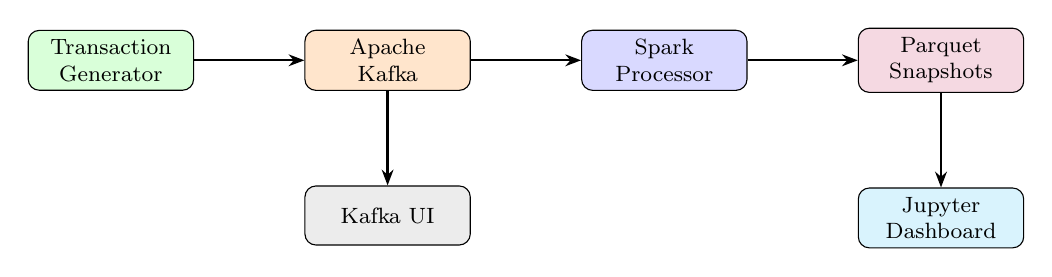
\begin{tikzpicture}[
    node distance=1.1cm and 1.4cm,
    box/.style={draw, rounded corners, minimum width=2.1cm, minimum height=0.75cm, align=center, font=\footnotesize},
    arr/.style={-{Stealth[length=2mm]}, thick}
  ]
    \node[box, fill=green!15] (gen) {Transaction\\Generator};
    \node[box, fill=orange!20, right=of gen] (kafka) {Apache\\Kafka};
    \node[box, fill=blue!15, right=of kafka] (spark) {Spark\\Processor};
    \node[box, fill=purple!15, right=of spark] (out) {Parquet\\Snapshots};
    \node[box, fill=cyan!15, below=1.2cm of out] (dash) {Jupyter\\Dashboard};
    \node[box, fill=gray!15, below=1.2cm of kafka] (ui) {Kafka UI};
    \draw[arr] (gen) -- (kafka);
    \draw[arr] (kafka) -- (spark);
    \draw[arr] (spark) -- (out);
    \draw[arr] (out) -- (dash);
    \draw[arr] (kafka) -- (ui);
  \end{tikzpicture}
  \vspace{0.8em}
  \begin{itemize}
    \item Topic: \texttt{bank-transactions} (3 partitions)
    \item Spark cluster: 1 master + 3 workers
    \item Full stack orchestrated with \textbf{Docker Compose}
  \end{itemize}
\end{frame}

\begin{frame}{Technology Stack}
  \begin{table}
    \centering
    \footnotesize
    \begin{tabular}{@{}ll@{}}
      \toprule
      \textbf{Layer} & \textbf{Technology} \\
      \midrule
      Messaging & Apache Kafka + Kafka UI \\
      Stream processing & Spark 3.5.3 Structured Streaming \\
      Simulation & Python 3.11 + NumPy + confluent-kafka \\
      Storage / serving & Parquet under \texttt{data/output/} \\
      Visualization & Jupyter + pandas + matplotlib \\
      Orchestration & Docker Compose \\
      \bottomrule
    \end{tabular}
  \end{table}
  \vspace{0.5em}
  \textbf{Monitoring URLs (local demo):}
  \begin{itemize}
    \item Jupyter: \url{http://localhost:8888} (token: \texttt{tp5fraud2026})
    \item Kafka UI: \url{http://localhost:8080}
    \item Spark Master UI: \url{http://localhost:8081}
  \end{itemize}
\end{frame}

\begin{frame}{Docker Compose Services (TP Requirement)}
  \begin{columns}[T]
    \column{0.48\textwidth}
    \textbf{Required services — all implemented:}
    \begin{enumerate}
      \item \texttt{transaction-generator}
      \item \texttt{kafka} + \texttt{kafka-init}
      \item \texttt{kafka-ui}
      \item \texttt{spark-master}
      \item \texttt{spark-worker-1/2/3}
      \item \texttt{spark-processor}
      \item \texttt{jupyter}
    \end{enumerate}
    \column{0.52\textwidth}
    \textbf{Deliverables in repository:}
    \begin{itemize}
      \item \texttt{README.md}
      \item \texttt{getting\_started.md}
      \item \texttt{docker-compose.yml}
      \item \texttt{src/transaction\_generator.py}
      \item \texttt{src/spark\_processor.py}
      \item \texttt{notebooks/fraud\_dashboard.ipynb}
      \item \texttt{docs/architecture.md}
    \end{itemize}
  \end{columns}
\end{frame}

%======================================================================
\section{Transaction Simulation}

\begin{frame}{Population Model}
  \textbf{Specification targets:}
  \begin{itemize}
    \item $N = 100{,}000$ Bank X clients (\texttt{client\_******})
    \item $M = 200{,}000$ external users — banks A \& B (\texttt{user\_a\_*}, \texttt{user\_b\_*})
  \end{itemize}
  \textbf{Development run (laptop-friendly):} $N{=}500$, $M{=}1{,}000$ via env vars.
  \vspace{0.5em}
  \textbf{Per-individual attributes:}
  \begin{itemize}
    \item Income $I_i$: power law $P(I) \propto I^{-2}$ on $[1{,}000;\ 1{,}000{,}000]$ MRU
    \item Spending $S_i \sim \mathcal{U}[I_i/1000,\ I_i/100]$
    \item Balance $B_i \sim \mathcal{U}[0,\ 3 I_i]$
    \item Frequency $f_i = I_i / S_i$ (tx/month)
    \item Per-second probability: $p_i = f_i / (30 \times 24 \times 3600)$
  \end{itemize}
\end{frame}

\begin{frame}{Transaction Generation Logic}
  \textbf{Every second:}
  \begin{enumerate}
    \item Bernoulli trial per user with probability $p_i \times \text{peak\_multiplier}$
    \item Random receiver among $N{+}M$ users
    \item Amount $A \sim \mathcal{U}[S_i - 2\sigma,\ S_i + 2\sigma]$, $\sigma = S_i/2$
    \item Reject if $A > B_i$ (insufficient funds); update balances
    \item Optional fraud injection (\texttt{tx\_type = fraud\_alert})
    \item Publish JSON batch to Kafka
  \end{enumerate}
  \vspace{0.4em}
  \textbf{JSON message format (Bank X spec):}
  \begin{lstlisting}[style=py,basicstyle=\ttfamily\tiny]
{
  "msg_entity": "bank_X", "app_type": "mobile_app",
  "send_entity": "bank_X", "receive_entity": "bank_A",
  "send_id": "client_000235", "receive_id": "user_a_000248",
  "amount": 18.87, "date": "2026-05-21T01:36:32Z",
  "tx_type": "transfer", "tx_id": "uuid-here"
}
  \end{lstlisting}
\end{frame}

%======================================================================
\section{Stream Processing}

\begin{frame}{Spark Structured Streaming Processor}
  \textbf{Design:} single Kafka consumer + \texttt{foreachBatch} (10\,s trigger)
  \begin{itemize}
    \item Parse JSON $\rightarrow$ event-time column
    \item Append micro-batches to \texttt{tx\_history}
    \item Recompute aggregates on history each batch
    \item Write Parquet snapshots for the dashboard
    \item Checkpoint: \texttt{checkpoints/processor/}
  \end{itemize}
  \vspace{0.4em}
  \textbf{Per-user perspectives:} \texttt{sent} and \texttt{received} (union)
\end{frame}

\begin{frame}{Computed Metrics (TP §2.1)}
  \footnotesize
  \begin{table}
    \centering
    \begin{tabular}{@{}ll@{}}
      \toprule
      \textbf{Category} & \textbf{Implementation} \\
      \midrule
      Avg amount sent/received & Sliding windows: 3h, 7d, 3w (21d), 3mo (90d) \\
      Transaction counts & Same windows (\texttt{tx\_count}) \\
      Distinct receivers/senders & \texttt{approx\_count\_distinct(counterparty)} \\
      Lifetime totals & \texttt{total\_amount}, \texttt{tx\_count} \\
      Lifetime avg h/d/w/mo & Derived from first/last event time \\
      Recent activity & Last micro-batch (dashboard filters 10\,s) \\
      Recent users & Top 20 by \texttt{last\_seen} \\
      \bottomrule
    \end{tabular}
  \end{table}
  \vspace{0.3em}
  \normalsize
  \textbf{Window configuration:}
  \begin{itemize}
    \item 3h window, slide 30 min \quad
    \item 7d / 1h \quad
    \item 21d / 6h \quad
    \item 90d / 1d
  \end{itemize}
\end{frame}

\begin{frame}[fragile]{Processor Execution Logs}
  \textbf{Spark processor (Docker logs) — successful batches:}
  \begin{lstlisting}[basicstyle=\ttfamily\footnotesize]
Streaming processor started.
Batch 0 processed OK
Batch 1 processed OK
Batch 2 processed OK
...
Batch 6 processed OK
  \end{lstlisting}
  \textbf{Transaction generator (sample):}
  \begin{lstlisting}[basicstyle=\ttfamily\footnotesize]
Starting generator N=500 M=1000 total=1500 topic=bank-transactions
tick=10 batch_size=1 total_sent=3
tick=20 batch_size=0 total_sent=6
  \end{lstlisting}
  \textit{Note:} Throughput scales with $N{+}M$ and \texttt{PEAK\_MULTIPLIER}; production target uses $N{=}100$k, $M{=}200$k.
\end{frame}

%======================================================================
\section{Live Dashboard}

\begin{frame}{Jupyter Dashboard Features}
  \textbf{Notebook:} \texttt{notebooks/fraud\_dashboard.ipynb}
  \begin{itemize}
    \item Reads latest Parquet snapshots from \texttt{/workspace/data/output/}
    \item \textbf{Last $\sim$10 seconds} of transactions (with fallback to latest batch)
    \item \textbf{Last 20 active users} with \texttt{last\_seen} timestamp
    \item Merged per-user table: lifetime + windowed metrics (3h, 7d, 3w, 3mo)
    \item Bar chart of amounts; \texttt{anomaly} flag (HIGH / FRAUD)
    \item Auto-refresh every 5\,s (configurable); manual \textbf{Refresh} button
  \end{itemize}
\end{frame}

\begin{frame}{Dashboard Results — Recent Users}
  \textbf{Observed at runtime} (Spark + generator active, dev population 1,500 users):
  \begin{table}
    \centering
    \footnotesize
    \begin{tabular}{@{}lc@{}}
      \toprule
      \textbf{user\_id} & \textbf{last\_seen (UTC)} \\
      \midrule
      client\_000235 & 2026-05-21 01:36:32 \\
      client\_000252 & 2026-05-21 01:36:32 \\
      user\_a\_000248  & 2026-05-21 01:36:12 \\
      client\_000407 & 2026-05-21 01:36:12 \\
      \bottomrule
    \end{tabular}
  \end{table}
  \vspace{0.4em}
  Mix of Bank X clients and external bank A users — network crosses entity boundaries as required.
\end{frame}

\begin{frame}{Dashboard Results — Per-User Metrics (Sample)}
  \footnotesize
  \textbf{Merged summary (excerpt from notebook output):}
  \begin{table}
    \centering
    \begin{tabular}{@{}lrrrr@{}}
      \toprule
      \textbf{user\_id} & \textbf{3h sent avg} & \textbf{3h sent cnt} & \textbf{3h recv avg} & \textbf{distinct} \\
      \midrule
      client\_000235 & 18.87 & 1 & --   & 1 receiver \\
      client\_000252 & --    & -- & 18.87 & 1 sender \\
      user\_a\_000248  & --    & -- & 14.87 & 1 sender \\
      client\_000407 & 14.87 & 1 & --   & 1 receiver \\
      \bottomrule
    \end{tabular}
  \end{table}
  \vspace{0.3em}
  \normalsize
  \begin{itemize}
    \item Lifetime metrics mirror windowed values early in the run
    \item Separate sent vs.\ received statistics per TP specification
    \item \texttt{distinct\_counterparties} populated for network analysis
  \end{itemize}
\end{frame}

\begin{frame}{Dashboard Results — Sliding Window Detail (3h)}
  \footnotesize
  \textbf{Windowed table for active users (3-hour sliding windows):}
  \begin{table}
    \centering
    \begin{tabular}{@{}llrrrl@{}}
      \toprule
      \textbf{user\_id} & \textbf{dir.} & \textbf{avg} & \textbf{cnt} & \textbf{dist.} & \textbf{window\_end} \\
      \midrule
      client\_000252 & received & 18.87 & 1 & 1 & 2026-05-21 04:00 \\
      client\_000407 & sent     & 14.87 & 1 & 1 & 2026-05-21 04:30 \\
      client\_000235 & sent     & 18.87 & 1 & 1 & 2026-05-21 04:00 \\
      user\_a\_000248  & received & 14.87 & 1 & 1 & 2026-05-21 03:30 \\
      \bottomrule
    \end{tabular}
  \end{table}
  \vspace{0.3em}
  \normalsize
  Multiple overlapping windows per user illustrate \textbf{sliding-window} behavior required by the TP.
\end{frame}

\begin{frame}{Anomaly Highlighting}
  \textbf{Fraud detection aids in dashboard:}
  \begin{itemize}
    \item Generator injects \texttt{fraud\_alert} transactions (high amount vs.\ income)
    \item Column \texttt{anomaly}: \textbf{HIGH} if amount $\geq$ 95th percentile of batch
    \item Column \texttt{anomaly}: \textbf{FRAUD} for \texttt{tx\_type == fraud\_alert}
    \item Bar chart: red bars for fraud, blue for normal transfers
  \end{itemize}
  \vspace{0.5em}
  \textbf{Example normal transfer amounts observed:} 14.87 -- 18.87 MRU (consistent with spending model $S_i$).
\end{frame}

%======================================================================
\section{Deployment \& Demo}

\begin{frame}{How to Run the Full Stack}
  \begin{enumerate}
    \item \texttt{cd TP5\_BigData}
    \item \texttt{docker compose up -d --build}
    \item Wait for Kafka healthy + Spark batches (\texttt{Batch X processed OK})
    \item Open Jupyter: \url{http://localhost:8888} — token \texttt{tp5fraud2026}
    \item Run all cells in \texttt{fraud\_dashboard.ipynb}
  \end{enumerate}
  \vspace{0.4em}
  \textbf{Production-scale simulation:}
  \begin{lstlisting}[style=py,basicstyle=\ttfamily\footnotesize]
N_CLIENTS=100000 M_EXTERNAL=200000 PEAK_MULTIPLIER=10 docker compose up -d
  \end{lstlisting}
\end{frame}

\begin{frame}{Fault Tolerance \& Scalability}
  \textbf{Implemented mechanisms:}
  \begin{itemize}
    \item Kafka topic with 3 partitions (parallelism)
    \item Spark streaming checkpoints (\texttt{checkpoints/processor/})
    \item \texttt{restart: unless-stopped} on generator and processor
    \item Vectorized NumPy simulation (scalable to large $N{+}M$)
    \item Distributed Spark cluster (3 workers)
  \end{itemize}
  \vspace{0.4em}
  \textbf{Demonstrated in class demo:}
  \begin{itemize}
    \item Services recover after disk cleanup and Docker restart
    \item Dashboard updates as new Parquet snapshots land
  \end{itemize}
\end{frame}

%======================================================================
\section{Conclusion}

\begin{frame}{Compliance with TP Specification}
  \begin{columns}[T]
    \column{0.5\textwidth}
    \textbf{Fully addressed:}
    \begin{itemize}
      \item Docker infrastructure (6+ services)
      \item Realistic transaction generator
      \item Kafka + Spark streaming pipeline
      \item Windowed \& lifetime metrics
      \item Live Jupyter dashboard
      \item English documentation
    \end{itemize}
    \column{0.5\textwidth}
    \textbf{Documented trade-offs:}
    \begin{itemize}
      \item Dev population 500+1000 vs.\ 100k+200k
      \item Distinct-set \textit{delta} between windows (future work)
      \item 1000+ tx/s: architecture ready; full benchmark pending
    \end{itemize}
  \end{columns}
\end{frame}

\begin{frame}{Future Improvements}
  \begin{itemize}
    \item Explicit metric: change in distinct senders/receivers across windows
    \item Delta Lake for ACID upserts on lifetime state
    \item ML fraud scoring on top of aggregated features
    \item Kubernetes deployment + horizontal autoscaling
    \item Prometheus/Grafana for operational monitoring
  \end{itemize}
\end{frame}

\begin{frame}
  \centering
  \Large Thank you for your attention!\\
  \vspace{1em}
  \normalsize
  \textbf{Questions?}\\
  \vspace{0.8em}
  Repository: \textit{[GitHub/GitLab URL]}\\
  Commit: \textit{[evaluation hash]}\\
  \vspace{0.5em}
  \small SID45 — ESP Nouakchott — TP5 Collective Project
\end{frame}

\end{document}
